\documentclass{standalone}
\usepackage{tikz}
\tikzset{ block/.style = {draw, fill=white, very thick, rectangle, minimum height=1cm, minimum width=2cm},}
\begin{document}
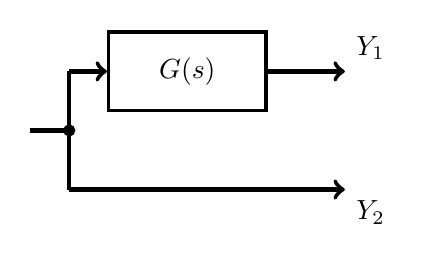
\begin{tikzpicture}[scale=2]
    \node[block](g){$G(s)$};
    \draw[-,ultra thick](-1,-0.375)--(-0.75,-0.375);
    \filldraw[black](-0.75,-0.375)circle(1pt);
    \draw[-,ultra thick](-0.75,-0.375)--(-0.75,0);
    \draw[->,ultra thick](-0.75,0)--(g.180);
    \draw[->,ultra thick](g.0)--(1,0)node[above right]{$Y_1$};
    \draw[-,ultra thick](-0.75,-0.375)--(-0.75,-0.75);
    \draw[->,ultra thick](-0.75,-0.75)--(1,-0.75)node[below right]{$Y_2$};
\end{tikzpicture}
\end{document}